%%%%%%%%%%%%%%%%%%%%%%%%%%%%%%%%%%%%%%%%%
%%% HYPERRIDE Reporting Template
%%%%%%%%%%%%%%%%%%%%%%%%%%%%%%%%%%%%%%%%%

\documentclass[letterpaper,12pt]{report}
\usepackage[pass]{geometry}
%\documentclass[11pt]{report}

\usepackage{hyperride}		% HYPERRIDE specific definitions and styles  
\usepackage[utf8]{inputenc}	% UTF8 package
\usepackage[T1]{fontenc}
\usepackage{textcomp}		% common special chars
\usepackage{amsmath}		% math formula
\usepackage{fancybox}
\usepackage{anyfontsize}	% fonts
\usepackage{lipsum}
\usepackage{float}
\usepackage[normalem]{ulem}
\usepackage{cleveref}
\usepackage[printonlyused]{acronym}
\hypersetup{
	pdftitle={0th Periodic Report},
	pdfauthor={[Names of co-authors (partners short names)]},
	pdfkeywords={Periodic Report, European Union (EU), H2020, Project, HYPERRIDE, GA 957788},
}
\usepackage{subfigure}
\usepackage{graphicx}
\usepackage{xcolor}
\usepackage{soul}
\sethlcolor{lightgray}
\usepackage[export]{adjustbox}
\usepackage{mdframed}
\usepackage{pdfpages}
\usepackage{comment}
\usepackage{multirow,array}
\def\todo#1{{\color{hyperridered}\textbf{TODO:} ``#1''}}
\def\hyperride{HYPERRIDE}

\graphicspath{ {graphics/} }

%%%%%%%%%%%%%%%%%%%%%%%%%%%%%%%%%%%%%%%%%
%%% Definitions
%%%%%%%%%%%%%%%%%%%%%%%%%%%%%%%%%%%%%%%%%

\begin{document}


\includepdf[pages=1]{./graphics/FP.pdf}

\mdfdefinestyle{code}{%
    linecolor=black,
    outerlinewidth=2pt,
    %roundcorner=20pt,
    innertopmargin=4pt,
    innerbottommargin=4pt,
    innerrightmargin=4pt,
    innerleftmargin=4pt,
        leftmargin = 4pt,
        rightmargin = 4pt
    backgroundcolor=black!10
    }

%%%%%%%%%%%%%%%%%%%%%%%%%%%%%%%%%%%%%%%%%
%%% URL style same as regular text
%%%%%%%%%%%%%%%%%%%%%%%%%%%%%%%%%%%%%%%%%
	
\urlstyle{same}

%%%%%%%%%%%%%%%%%%%%%%%%%%%%%%%%%%%%%%%%%
%%% Deliverable Information
%%%%%%%%%%%%%%%%%%%%%%%%%%%%%%%%%%%%%%%%%

% Project Meta Information
\ProjectFullTitle{Beacon Web Security Labs: Domain Takeover Attack Lab Setup}
\ProjectAcronym{HYPERRIDE}
\ProjectRefNo{957788}

% Report Number, use either "1", "2", or "3" for the corresponding reporting period
\delivNumber{0}

% Period covered by the report
\delivFrom{dd/mm/yyyy}
\delivTo{dd/mm/yyyy}

% Report Responsible Partner
\delivResponsible{AIT Austrian Institute of Technology (AIT)} 

% Report Version, Contractual and Actual Date, Dissemination Level, Type
\delivVersion{vn.n}
\ContractualDate{dd/mm/yyyy}
\ActualDate{dd/mm/yyyy}

% List of Main Authors (usually from the responsible partner)
\delivAuthor{[Names of co-authors (partners short names)]}

% List of Co-Authors (all other co-authors should be listed here)
\delivFPAuthor{[Names of co-authors (partners short names)]}

% Report Status
\delivStatus{d} %% d = draft, f = final, s = submitted

%%%%%%%%%%%%%%%%%%%%%%%%%%%%%%%%%%%%%%%%%
%%% Change Log
%%%%%%%%%%%%%%%%%%%%%%%%%%%%%%%%%%%%%%%%%

\istChange{dd/mm/yyyy}{v1.0}{Name (Partner short name)}{Draft report template}
\istChange{}{}{}{}

%%%%%%%%%%%%%%%%%%%%%%%%%%%%%%%%%%%%%%%%%
%%% Cover Page
%%%%%%%%%%%%%%%%%%%%%%%%%%%%%%%%%%%%%%%%%

%\makecover

%%%%%%%%%%%%%%%%%%%%%%%%%%%%%%%%%%%%%%%%%
%%% Table of Contents
%%%%%%%%%%%%%%%%%%%%%%%%%%%%%%%%%%%%%%%%%

\clearpage
\fancypagestyle{plain}{}
\settableofcontents
\tableofcontents
\clearpage

%%%%%%%%%%%%%%%%%%%%%%%%%%%%%%%%%%%%%%%%%
%%% Overview
%%%%%%%%%%%%%%%%%%%%%%%%%%%%%%%%%%%%%%%%%

\section*{Downloading Oracle VM Virtual Box}\label{sec:overview}
\addcontentsline{toc}{section}{Downloading Oracle VM Virtual Box}

VirtualBox will be the virtual machine software that is used to open the VM images and complete the lab. It is possible to complete the lab with other virtual machine software but it has been untested and so support for other virtual machine software will not be included in this lab document at this point in time.

Begin by downloading Oracle's VirtualBox software. The download links for VirtualBox can be found at the below website.

\url{https://download.virtualbox.org/virtualbox/7.0.18/VirtualBox-7.0.18-162988-Win.exe}

\subsection*{Windows Setup}\label{sec:Virtual-Machine-Windows-Setup}
\addcontentsline{toc}{subsection}{Windows Setup}

Select the hyperlink titled "Windows hosts" under the "VirtualBox x.x.xx platform packages" to begin the installation of the latest version of VirtualBox. This lab was created when VirtualBox 7.0.18 was the latest release, however, the steps provided should still apply to future versions of VirtualBox as well, the images shown may not be identical, however.

Once the download has completed, run the downloaded installer. The file name should be "VirtualBox-<version\_number>-Win.exe".

Run through the installer without changing anything. At the end, make sure the checkbox is selected to "Start Oracle VM VirtualBox x.x.xx after installation" then click the "Finish" button to complete the installation and open VirtualBox.

\subsection*{Linux Setup}\label{sec:Virtual-Machine-Linux-Setup}
\addcontentsline{toc}{subsection}{Linux Setup}

Select the hyperlink titled "Linux distributions" under the "VirtualBox <version\_number> platform packages" to navigate to the page containing Oracle's instructions for distribution specific instructions for downloading and installing VirtualBox.

Find your distribution and follow the instructions Oracle has provided.

If your distribution isn't shown on the website, please look into distribution specific instructions for your Linux distro. For example, if you are using Arch Linux, there is a VirtualBox page on the ArchWiki that provides an installation guide.

\section*{Downloading the Virtual Machine Image}
\addcontentsline{toc}{section}{Downloading the Virtual Machine Image}

The image file for this lab's VM can be found on this lab's page on the \href{https://sites.google.com/d/1s2NT4x8p2UBLm59LHOYuVmEUOx35X7U0/p/1abEx9crWZcozrGUZH595BVCAogd-K5A1/edit?authuser=1}{BEACON Website} or through the links below.

\url{https://drive.google.com/file/d/1X4gZaDfmjbE4BzVahDIaVkTIabQGSdYT/view?usp=drive_link}

\url{https://drive.google.com/file/d/1UaP4fSF32fG8sQ_aGR4oa8en9pArHVK7/view?usp=drive_link}

The files are 7.79 and 8.61 GB in size so the download may take a while depending on your internet speed.

\section*{Setting up the Virtual Machine}
\addcontentsline{toc}{section}{Setting up the Virtual Machine}

Once the image file is downloaded, open VirtualBox if it's not open already. The window that pops up should be titled "Oracle VM VirtualBox Manager" and should look similar to Figure~\ref{fig:VirtualBox_Manager} on page~\pageref{fig:VirtualBox_Manager}. This window will be where we setup the virtual machine that will be used in this lab.

\begin{figure}[!ht]
    \centering
    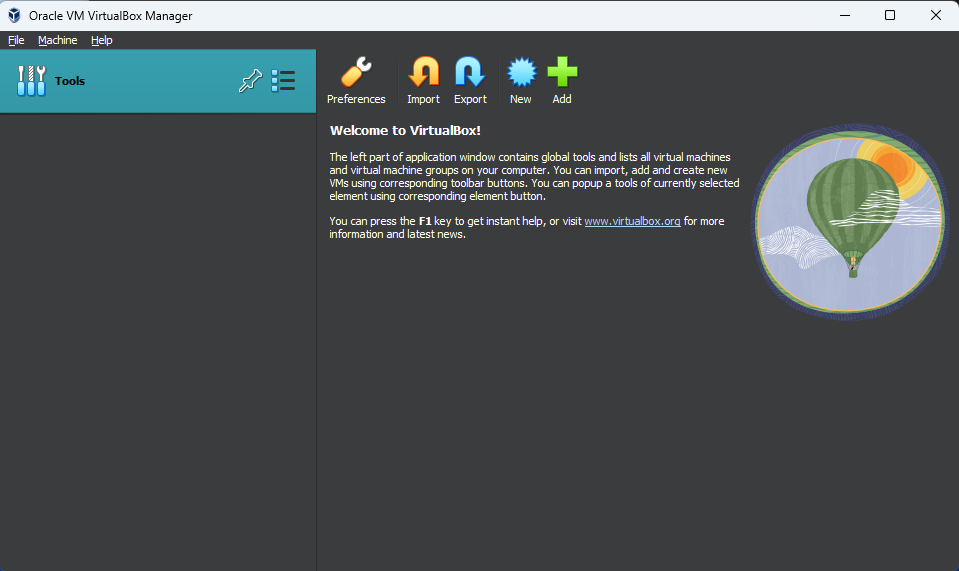
\includegraphics[width=0.4\columnwidth]{graphics/oracle_vm_virtualbox_manager.png}
    \caption{VirtualBox Manager}
    \label{fig:VirtualBox_Manager}
\end{figure}

From the VirtualBox Manager, click the "Import" button, found either on the home page under the Tools banner or in the menu bar under File > Import Appliance. This should open a new window that looks like Figure~\ref{fig:Import_Virtual_Appliance} on page~\pageref{fig:Import_Virtual_Appliance}.

Click the yellow folder icon with a green arrow pointing upwards on the middle-right side of the window to open your operating system's file picker. In this file picker, navigate to where you downloaded the virtual machine .ova image and select "swxss-lab-attacker.ova" and then select "Open."

\begin{figure}[!ht]
    \centering
    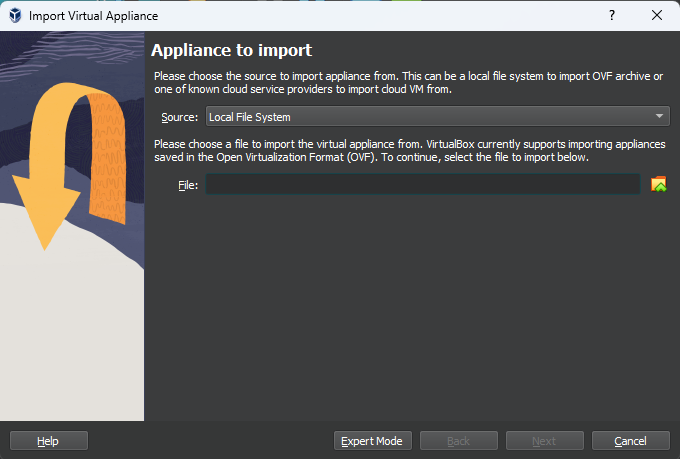
\includegraphics[width=0.4\columnwidth]{graphics/import_virtual_appliance.png}
    \caption{Import Virtual Appliance Window}
    \label{fig:Import_Virtual_Appliance}
\end{figure}

The VM image should now be imported and appear on the left side of the VirtualBox Manager. Select the VM and open the Settings menu. Navigate to the Network settings of the VM and make sure Adapter 1 is enabled, attached to the internal network, and has been renamed to "swxss-network" to make sure the lab will be conducted on a separate internal network.

It's important that we we do this to put the VM in an isolated environment in order to minimize the risk of an outside attacker accessing the vulnerable website used in this lab.

\begin{figure}[!bh]
    \centering
    
\includegraphics[width=0.3\columnwidth]{graphics/vm_start_button.png}
    \caption{The Start button for VM instances}
    \label{fig:VM_Start_Button}
\end{figure}

\textbf{Repeat the same process for the "defender-vm.ova" virtual machine image file.}

The final step in setting up the virtual machines is to actually start them. It's recommended to start the attacker VM first.

To start the attacker VM, select it from the list of virtual machines on the left side of the VirtualBox Manager and either double click it or, click the green "Start" button as shown in Figure~\ref{fig:VM_Start_Button} on page~\pageref{fig:VM_Start_Button}.

For the defender VM, we'll be starting it in a headless state. To do so, select the defender VM from the menu on the left, click the small arrow to the right of the start button, and then select the "headless start" option.

The username and password for each VM is "swxss".

\end{document}

%%%%%%%%%%%%%%%%%%%%%%%%%%%%%%%%%%%%%%%%%